\chapter{Generalization}


\begin{enumerate}
    \item Our real quest is to discover \textbf{general patterns} on the basis of which we can make accurate predictions even on new examples drawn from the same underlying population.

    \item The difference between our fit on the training data and our fit on the test data is called the \textbf{generalization gap}\indexlabel{generalization gap} and when this is large, we say that our models \textbf{overfit}\indexlabel{overfit} to the training data.

    \item In extreme cases of overfitting, we might exactly fit the training data, even when the test error remains significant. 
    
    \item In the classical view, the interpretation is that our models are too complex, requiring that we either shrink the number of features, the number of nonzero parameters learned, or the size of the parameters as quantified.
\end{enumerate}

\section{Regularization Techniques} \label{regularization techniques}

\begin{enumerate}
    \item our models are typically expressive enough to perfectly fit every training example, even in datasets consisting of millions

    \item we might think that this setting lies on the far right extreme of the model complexity axis, and that any improvements in generalization error must come by way of regularization, either by reducing the complexity of the model class, or by applying a penalty, severely constraining the set of values that our parameters might take.

    \item it is often the case that despite fitting the training data perfectly, we can actually \textbf{reduce the generalization} error further by \textbf{making the model even more expressive}, e.g., adding layers, nodes, or training for a larger number of epochs.

    \item the pattern relating the generalization gap to the complexity of the model (as captured, for example, in the depth or width of the networks) can be non-monotonic, with greater complexity hurting at first but subsequently helping in a so-called \textbf{“double-descent” pattern}\indexlabel{double-descent pattern}

    \item because neural networks are over-parametrized, possessing many more parameters than are needed to fit the training data, they tend to \textbf{interpolate} the training data (fitting it perfectly) and thus behave, in some ways, more like nonparametric models.

    \item in the limit, as multilayer perceptrons with randomly initialized weights grow infinitely wide, they become equivalent to (nonparametric) kernel methods for a specific choice of the kernel function (essentially, a distance function), which they call the neural tangent kernel.

    
\end{enumerate}



\subsection{Weight Decay \cite{dnn-1}}\label{regularization techniques: Weight Decay}

\begin{enumerate}[itemsep=0.2cm]
    \item Rather than directly manipulating the \textbf{number of parameters}, weight decay, operates by restricting the \textbf{values} that the parameters can take.

    \item The most common method for ensuring a small weight vector is to add its norm as a \textbf{penalty term} to the problem of minimizing the loss.

    \item We replace our original objective, \textbf{minimizing the prediction loss on the training labels}, with new objective, \textbf{minimizing the sum of the prediction loss and the penalty term}.

    \item Absent early stopping, it is possible that just like the number of layers or number of nodes (in deep learning) or the distance metric (in 1-nearest neighbor), these methods may lead to better generalization \textbf{NOT} because they meaningfully constrain the power of the neural network but rather because they somehow encode inductive biases that are better compatible with the patterns found in datasets of interests. 

    \item Example:
    \begin{customTableWrapper}{2}
        \begin{table}[H]
            \centering
            \begin{tabular}{l l}
                features & $\mathbf{x}^{(i)}$ \\

                label & $y^{(i)}$ \\

                data example & $i$ \\

                weight and bias parameters & $(\mathbf{w}, b)$ \\
            
                Linear Function & $f(\mathbf{x}) = \mathbf{w}^\top \mathbf{x}$ \\
    
                Loss Fucntion & $L(\mathbf{w}, b) = \dfrac{1}{n}\dsum_{i=1}^n \dfrac{1}{2}\left(\mathbf{w}^\top \mathbf{x}^{(i)} + b - y^{(i)}\right)^2$ \\

                regularization constant & $\lambda$ ($\lambda \geq 0$)\\

            \end{tabular}
        \end{table}
    \end{customTableWrapper}

    \item Now, if our weight vector grows too large, our learning algorithm might focus on minimizing the weight norm $\dnorm{\mathbf{w}}^2$ rather than minimizing the training error. That is exactly what we want.

    \item Penalized loss function: $L(\mathbf{w}, b) + \dfrac{\lambda}{2} \dnorm{\mathbf{w}}^2$
    \begin{enumerate}
        \item For $\lambda = 0$, we recover our original loss function.

        \item For $\lambda > 0$, we restrict the size of $\dnorm{\mathbf{w}}$.

        \item $1/2$ is for mathematical convenience during derivative

    \end{enumerate}

\end{enumerate}



\subsubsection{Lasso Regression/ $\ell_1$-regularization \cite{dnn-1,geeksforgeeks.org/regularization-in-machine-learning}} \label{l1 regularization/ Lasso Regression}

\begin{enumerate}
    \item A regression model which uses the L1 Regularization technique is called \textbf{LASSO (Least Absolute Shrinkage and Selection Operator)} regression.

\end{enumerate}


\[
    Cost = L(\mathbf{w}, b) + \dfrac{\lambda}{2} \dsum_{i=1}^m \dabs{w_i}
\]


\subsubsection{Ridge Regression/ $\ell_2$-regularization \cite{dnn-1,geeksforgeeks.org/regularization-in-machine-learning}} \label{l1 regularization/ Ridge Regression}


\[
    Cost 
    = L(\mathbf{w}, b) + \dfrac{\lambda}{2} \mathbf{w}^\top\mathbf{w}
    = L(\mathbf{w}, b) + \dfrac{\lambda}{2} \|\mathbf{w}\|^2
\]


\subsubsection{Elastic Net Regression/ $\ell_2$ \& $\ell_2$-regularization \cite{dnn-1,geeksforgeeks.org/regularization-in-machine-learning}} \label{Elastic Net Regression}





\section{Early Stopping \cite{dnn-1}} \label{Early Stopping}

\begin{enumerate}
    \item While deep neural networks are capable of fitting arbitrary labels, even when labels are assigned incorrectly or randomly, this capability only emerges over many iterations of training. 

    \item in the setting of label noise, neural networks tend to fit cleanly labeled data first and only subsequently to interpolate the mislabeled data.

    \item whenever a model has fitted the cleanly labeled data but not randomly labeled examples included in the training set, it has in fact generalized

    \item Here, rather than directly constraining the values of the weights, one constrains the number of epochs of training.

    \item The most common way to determine the stopping criterion is to monitor validation error throughout training (typically by checking once after each epoch) and to cut off training when the validation error has not decreased by more than some small amount $\epsilon$ for some number of epochs. This is sometimes called a \textbf{patience criterion} \indexlabel{patience criterion}.

    \item another benefit of early stopping is the \textbf{time saved}

    \item when there is no label noise and datasets are realizable (the classes are truly separable, e.g., distinguishing cats from dogs), early stopping tends not to lead to significant improvements in generalization.\\
    On the other hand, when there is label noise, or intrinsic variability in the label (e.g., predicting mortality among patients), early stopping is crucial.\\
    Training models until they interpolate noisy data is typically a bad idea.
\end{enumerate}



\section{Dropout \cite{dnn-1,gfg-dropout-in-neural-networks,medium/towardsdatascience.com/dropout-in-neural-networks-47a162d621d9}} \label{Dropout}


\begin{table}[H]
    \begin{minipage}{0.45\linewidth}
        \begin{figure}[H]
            \centering
            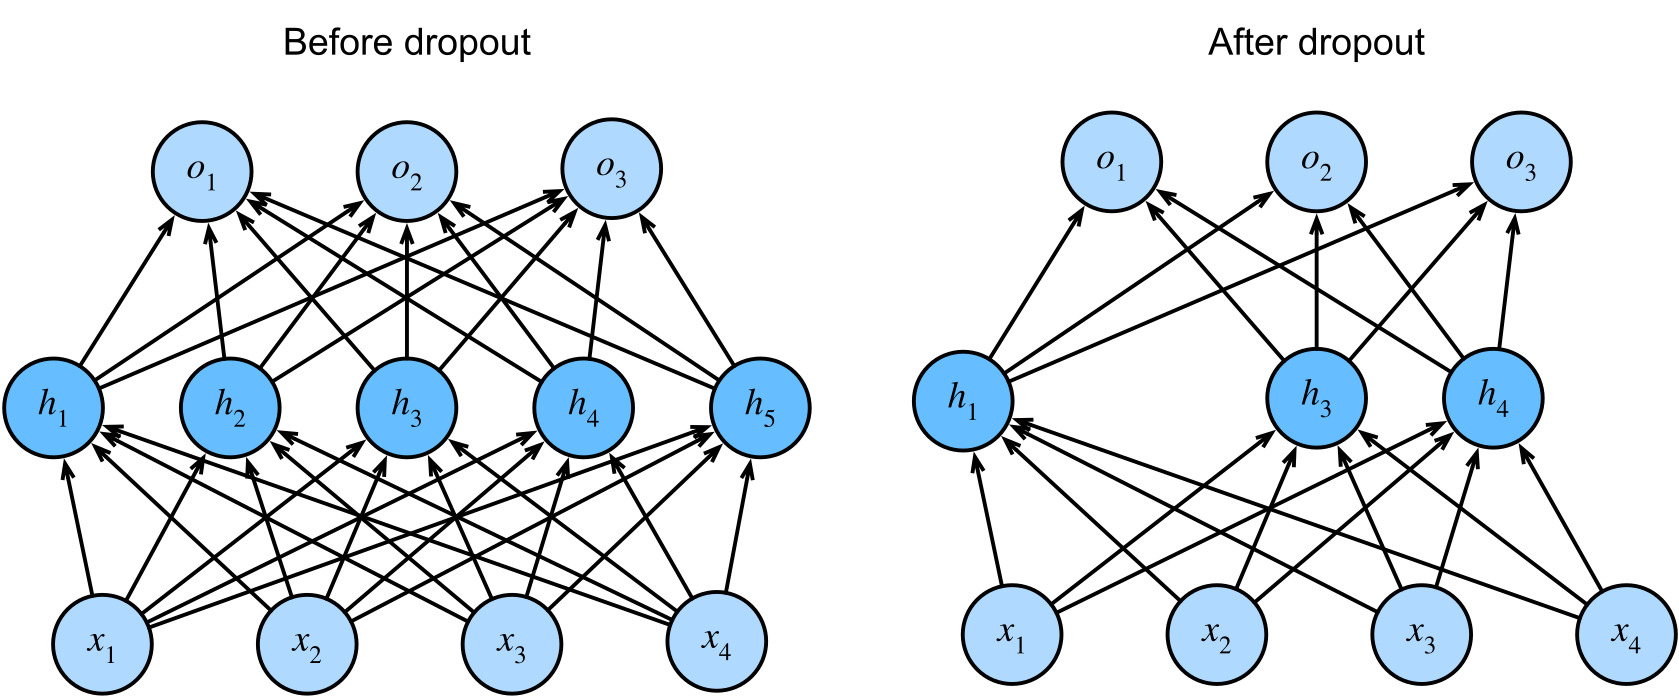
\includegraphics[width=\linewidth, height=3.5cm, keepaspectratio]{Pictures/deep_neural_networks/dropout.jpg}
            \caption{Dropout Example \cite{dnn-1}}
        \end{figure}
    \end{minipage}
    \hfill
    \begin{minipage}{0.45\linewidth}
        \begin{figure}[H]
            \centering
            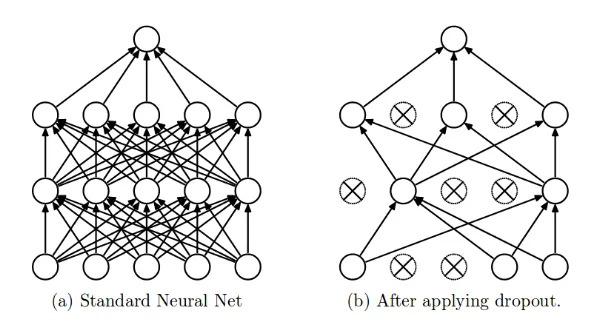
\includegraphics[width=\linewidth, height=3.5cm, keepaspectratio]{Pictures/layers/dropout.jpg}
            \caption{Dropout Layer \cite{medium/towardsdatascience.com/dropout-in-neural-networks-47a162d621d9}}
        \end{figure}
    \end{minipage}
\end{table}


\begin{enumerate}
    \item to close the gap between train and test performance, we should aim for a simple model.\\ 
    Simplicity can come in the form of a small number of dimensions.

    \item Another useful notion of simplicity is smoothness, i.e., that the function should not be sensitive to small changes to its inputs.\\
    For instance, when we classify images, we would expect that adding some random noise to the pixels should be mostly harmless.

    \item The idea, called \textbf{dropout}, involves injecting noise while computing each internal layer during forward propagation, and it has become a standard technique for training neural networks. 
    
    \item The method is called dropout because we literally \textbf{drop out} some neurons during training.\\
    Throughout training, on each iteration, standard dropout consists of zeroing out some fraction of the nodes in each layer before calculating the subsequent layer.

    \item neural network overfitting is characterized by a state in which each layer relies on a specific pattern of activations in the previous layer, calling this condition \textbf{co-adaptation} \indexlabel{co-adaptation}.

    \item One idea is to \textbf{inject noise} in an \textit{unbiased manner} so that the expected value of each layer—while fixing the others—equals the value it would have taken absent noise.\\
    In \textbf{Bishop’s work}, he added \textbf{Gaussian noise} to the inputs to a linear model.\\
    At each training iteration, he added noise sampled from a distribution with mean zero $\epsilon \sim \mathcal{N}(0,\sigma^2)$ to the input $\mathbf{x}$, yielding a perturbed point $\mathbf{x}' = \mathbf{x} + \epsilon$. \\
    In expectation, $E[\mathbf{x}'] = \mathbf{x}$.

    \item In \textbf{standard dropout regularization}, one \textbf{zeros out} some fraction of the nodes in each layer and then \textbf{debiases} each layer by normalizing by the fraction of nodes that were retained (not dropped out).\\
    In other words, with dropout probability $p$, each intermediate activation $h$ is replaced by a random variable $h'$ as follows:
    \[
        h' =
        \begin{dcases}
            0 & \textrm{ with probability } p \\
            \dfrac{h}{1-p} & \textrm{ otherwise}
        \end{dcases}
    \]
    By design, the expectation remains unchanged, i.e., $E[h'] = h$

    \item All the forward and backwards connections with a dropped node are temporarily removed, thus creating a new network architecture out of the parent network. 
    
    \item In every iteration, you will work on a smaller neural network than the previous one and therefore, it approaches \textbf{regularization}.

    \item Dropout helps in \textbf{shrinking} the squared norm of the weights and this tends to a reduction in overfitting.

\end{enumerate}

\vspace{0.3cm}
\noindent\textbf{NOTE}:
\begin{enumerate}[itemsep=0.2cm]
    \item \textbf{Training Phase}:
    \begin{enumerate}
        \item the dropped nodes are still part of the network and not permanently dropped. 
    
        \item the dropped neurons might be used in another epoch for fitting
    \end{enumerate}

    \item \textbf{Testing Phase}:
    \begin{enumerate}
        \item during testing phase, neurons are not dropped at all

        \item all neurons are used, and the weights are usually scaled accordingly to account for the dropout that occurred during training
    \end{enumerate}
\end{enumerate}
















